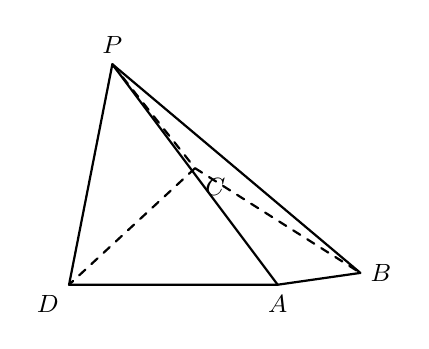
\begin{tikzpicture}[thick,line cap=round,line join=round,
  every node/.style={font=\small}]
  \coordinate (P) at (0,2.8);
  \coordinate (D) at (-.55,0);
  \coordinate (A) at (2.1,0);
  \coordinate (B) at (3.15,.15);
  \coordinate (C) at (1.05,1.48);
  \draw (P)--(D)--(A)--(B)--(P);
  \draw (P)--(A);
  \draw[dashed] (P)--(C) (C)--(D) (C)--(B);
  \node[above] at (P) {$P$};
  \node[below left] at (D) {$D$};
  \node[below] at (A) {$A$};
  \node[right] at (B) {$B$};
  \node[below right] at (C) {$C$};
\end{tikzpicture}
